\section{Marginal Surprise}
The smart reader suddenly notes that the definition of subgraph probability is a natural way to measure the significance of the hypothesis that the particular observed value of subgraph \emph{internal} density is higher than the average graph density.
This concept relates to the degree to which subgraph nodes relates each other rather than to external nodes.

An opposite idea is to see to what level of significance the fraction of links that a subgraph is throwing \emph{outside} is smaller than what expected on the basis of the global graph properties.
In this respect, similarly to what is done for the subgraph probability in Eq.~\ref{eq:surprise} one may want to know what is the probability of observing the intercluster density of the subgraph $\mathcal{G}_c$, specified by

\begin{equation}
\rho_{\textrm{out}}(\mathcal{G}_c)=\frac{m_c^{\textrm{out}}}{n_c(n-n_c)}
\end{equation}

less than or equal to a fixed value in a subgraph drawn randomly from a graph with a given density $\rho=m/p$.
This concept is expressed in probabilistic form in the following equation:
\begin{align}\label{eq:centripetalsignificance}
\Pr[m^{\textrm{out}}_c \leq q ] &= \sum \limits_{i=0}^{q} \frac{\binom{m}{i}\binom{p-m}{n_c(n-n_c)-i)}}{\binom{p}{n_c(n-n_c)}} \nonumber \\ 
& = \sum \limits_{i=0}^{q} \frac{\binom{n_c(n-n_c)}{i}\binom{p-n_c(n-n_c)}{m-i}}{\binom{p}{m}}
\end{align}

But there is a refinement for equation \ref{eq:centripetalsignificance}:
\begin{align}
\Pr[m^{\textrm{out}}_c \leq q | m_c =r] &= \sum \limits_{i=0}^{q} \dfrac{\binom{m-r}{i} \binom{p-p_c - (m-r)}{n_c(n-n_c) - i}}{\binom{p-p_c}{n_c(n-n_c)}} \\
 &=  \sum \limits_{i=0}^{q} \dfrac{\binom{n_c(n-n_c)}{i}\binom{p-p_c-n_c(n-nc)}{m-r-i)}}{\binom{p-p_c}{m-r}}\\
  &=  1- \sum \limits_{i=q}^{m} \dfrac{\binom{n_c(n-n_c)}{i}\binom{p-p_c-(n_c(n-nc))}{m-r-i}}{\binom{p-p_c}{m-r}}
\end{align}

One wants to find a subgraph $\mathcal{G}=(\mathcal{V},\mathcal{E})$ with $|\mathcal{V}|=n_c$ nodes out of a graph with $n$ nodes, partitions the total number of edges in the graph $G$ as the sum of three contributes, $m_c=|\mathcal{E}|$ that is the number of edges of $\mathcal{G}$, the number of edges that $\mathcal{G}$ projects to the rest of the graph, that we call $m^{\textrm{out}}_c$ and the number of edges that have no endpoint in $\mathcal{G}$ that we call $m_{\tilde{c}}$:

\begin{equation}
m = m_c + m^{\textrm{out}}_c + m_{\tilde{c}}
\end{equation}

For fixed $m$, the larger $m_c$ is, the stricter is the upper bound on $m^{\textrm{out}}_c$. Hence a better test of how probable a particular value of $m^{\textrm{out}}_c$ is, would involve computing the probability under the assumption that $m_c$ is fixed as its observed value; that is, a better test would involve computing the conditional probability $\Pr[m^{\textrm{out}}_c \leq q | m_c =r]$.

To compute this probability, it is sufficient to reduce the graph by $p$ pairs of nodes of which $r$ are edges, and then to compute the probability of observing $q$ or fewer edges in a randomly drawn set containing $L(n,N)$ pairs of nodes. This probability is given by the expression:

\begin{align}\label{eq:hyperrefinement}
\Pr[m^{\textrm{out}}_c \leq q | m_c =r] &= \sum \limits_{i=0}^{q} \dfrac{\binom{m-r}{i} \binom{p-p_c - (m-r)}{n_c(n-n_c) - i}}{\binom{p-p_c}{n_c(n-n_c)}} \\
&=  \sum \limits_{i=0}^{q} \dfrac{\binom{n_c(n-n_c)}{i}\binom{(p-p_c)-(n_c(n-nc)))}{(m-r)-i)}}{\binom{(p-p_c)}{m-r}}
\end{align}


Figure \ref{fig:subgraphconditionalprobability} shows the settings of this problem. A random subgraph $\mathcal{G}$ is chosen, consisting in nodes $\{e,f,g,h\}$, the remaining nodes form the subgraph $G-\mathcal{G}$.
\begin{figure}[htb]
\centering
\begin{tikzpicture}
%\draw[help lines,step=1] (-4,-4) grid (8,4);
\draw [rectangle, black, draw, rounded corners=2ex,line width=0.25ex] (1.6,-0.5) rectangle (3.4,1.5);

\draw (1,0) -- (3,0);
\draw (2,1) -- (3,1) -- (2,0) -- (3,0) -- cycle;
\node [fill=gray!30, radius=1ex, draw, circle, inner sep=2pt] at (2,1) {$e$};
\node [fill=gray!30, radius=1ex, draw, circle, inner sep=2pt] at (3,1) {$f$};
\node [fill=gray!30, radius=1ex, draw, circle, inner sep=2pt] at (2,0) {$g$};
\node [fill=gray!30, radius=1ex, draw, circle, inner sep=2pt] at (2,0) {$g$};
\node [fill=gray!30, radius=1ex, draw, circle, inner sep=2pt] at (3,0) {$h$};
\draw (0,1) -- (1,1);
\draw (1,1) -- (1,0);
\draw (1,0) -- (1,1);
\draw (1,1) -- (0,0);
\node [fill=gray!30, radius=1ex, draw, circle, inner sep=2pt] at (0,1) {$a$};
\node [fill=gray!30, radius=1ex, draw, circle, inner sep=2pt] at (1,1) {$b$};
\node [fill=gray!30, radius=1ex, draw, circle, inner sep=2pt] at (0,0) {$c$};
\node [fill=gray!30, radius=1ex, draw, circle, inner sep=2pt] at (1,0) {$d$};
\node at (2.5,1.75) {$\mathcal{G}$};
\node at (0.5,1.75) {{\color{red}$G-\mathcal{G}$}};
\draw [rectangle, red, draw, rounded corners=2ex,line width=0.25ex] (-0.4,-0.5) rectangle (1.4,1.5);
\node [] at (5.5,1) {$\Pr(\mathcal{G}) = \dfrac{\binom{6}{4} \binom{28-4}{10-6}}{\binom{28}{10}}$};
\node [] at (6.0,0) {$\approx 0.0121$};

\node [] at (9.5,1) {$m_c=4,p_c=6,n_c=4$};
\node [] at (9.5,0) {$p=28,m=10,n=8$};
\end{tikzpicture}
\caption{Probability for the subgraph $\mathcal{G}=(\mathcal{V},\mathcal{E})$ where $\mathcal{V}=\{e,f,g,h\}$ and $\mathcal{E}=\{(e,f),(f,g),(g,h),(e,h)\}$ to be randomly drawn from the graph $G$.}
\label{fig:subgraphconditionalprobability}
\end{figure}


This last formula corresponds to an urn model where the number of balls in the urn is $p-p_c$, the number of white balls in the urn is $n_c(n-n_c)$, the number of drawn balls is $m-r$ and the number of white extracted balls in $q$.

The probability of a partition is then the marginal distribution of Eq. \ref{eq:hyperrefinement}, obtained by summing over all values of $r$ from $0$ to $m$.

\begin{equation}
\mathcal{S}_m =  \sum \limits_{r=0}^m \Pr[m^{\textrm{out}}_c \leq q | m_c =r]
\end{equation}
